\subsubsection{Simple Actors \label{sec:simple_actors}}

Simple actors have workflow symbols that consist of a single (rather
than multiple) green-blue rectangle. They may also have an icon within the rectangle
to aid in their identification. The following actors are simple actors:
\begin{itemize}
\item{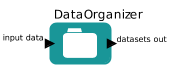
\includegraphics[width=2.5cm,height=1.3cm]{reflex_data_organiser_actor.png} - The {\tt DataOrganiser} actor.}
\item{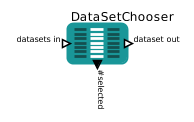
\includegraphics[width=2.5cm,height=1.6cm]{reflex_data_set_chooser_actor.png} - The {\tt DataSetChooser} actor (inside a composite actor).}
\item{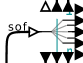
\includegraphics[width=1.6cm,height=0.8cm]{reflex_fits_router_actor.png} - The {\tt FitsRouter} actor} Redirects files according to their categories.
\item{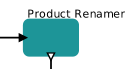
\includegraphics[width=1.8cm,height=1cm]{reflex_product_renamer_actor.png} - The {\tt ProductRenamer} actor.}
\item{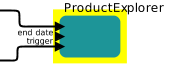
\includegraphics[width=2.2cm,height=1cm]{reflex_provenance_explorer_actor.png} - The {\tt ProductExplorer} actor (inside a composite actor).}
\end{itemize}

Access to the parameters for a simple actor is achieved by
right-clicking on the actor and selecting {\tt Configure Actor}. This
will open an ``Edit parameters'' window. Note that the {\tt Product Renamer}
actor is a jython script (Java implementation of the Python
interpreter) meant to be customised by the user (by double-clicking on
it).

